\documentclass[12pt]{article}


\usepackage[english,italian]{babel}

\usepackage{graphicx}
\usepackage{fancyhdr}
\usepackage{subfig}
\usepackage{float}

\usepackage[utf8]{inputenc}

\usepackage{hyperref}
\hypersetup{
  colorlinks,
  citecolor=gray,
  filecolor=brown,
  linkcolor=black,
  urlcolor=cyan
}

\usepackage{lastpage}

\usepackage{parcolumns}

\usepackage{listings}
\usepackage[usenames]{color}

\usepackage[a4paper,top=3cm,bottom=2cm,left=2cm,right=2cm] {geometry}

\usepackage[pdftex]{lscape}

\renewcommand{\familydefault}{\sfdefault}

\definecolor{editorGray}{rgb}{0.95, 0.95, 0.95}
\definecolor{editorOrange}{rgb}{1, 0.5, 0}
\definecolor{editorGreen}{rgb}{0, 0.6, 0}


\begin{document}

\begin{figure}
\centering

\includegraphics[scale=1.5]{images/Logo.png}
\end{figure} 

\title{ \textbf{{\Huge RESIDENCE AL MUGO}}\vspace{2cm} \\ {\Huge Tecnologie Web \\ Relazione del progetto} \\ {\vspace{1cm} \Large Anno Accademico 2016/2017} }
 
\author{
\begin{tabular}{r|l}
\textbf{Componenti} & Lahmer Abdelilah\\
&Maran Matteo\\
&Zanon Edoardo \vspace{0.3cm} \\
\textbf{Indirizzo Web} & \url{http://tecweb2016.studenti.math.unipd.it/edzanon}\vspace{0.3cm} \\
\textbf{Email responsabile} & \href{mailto:edoardo.zanon@studenti.math.unipd.it}{edoardo.zanon@studenti.math.unipd.it}
\end{tabular}
\vspace{2cm} 
}

\maketitle
\thispagestyle{empty}


\newpage


\pagestyle{fancy}
\lhead{}
\lfoot{\emph{\large Residence Al Mugo}} 
\cfoot{}
\rfoot{Pagina \thepage\ di \pageref{LastPage}}
\renewcommand{\footrulewidth}{0.5pt}

\tableofcontents

\newpage

\section{Abstract}

Per il progetto di tecnologie web il gruppo PamperoWeb ha scelto di presentare un sito per il RESIDENCE AL MUGO, situato a Siror in provincia di Trento. Tale residence possiede già un sito ma abbiamo pensato di migliorarlo rendendolo accessibile con le specifiche apprese durante il corso di studi. Il nostro sito permette agli utenti di avere un quadro generale sul residence, la sua ubicazione e descrizione. Inoltre permette di registrarsi con la possibilità di prenotare un appartamento per un dato periodo oltre a mettere a disposizione una lato amministratore che consente la gestione delle prenotazioni dei clienti, quella degli appartamenti e delle prenotazioni; con rispettivi check in, check out e fatture per gli utenti.

\newpage

\section{Progettazione}

\subsection{Struttura}

\subsubsection{Organizzazione cartelle}
I file che compongono il sito sono organizzati su 3 cartelle:
\begin{itemize}
\item \textbf{directory generale:} contiene la pagina \textit{index.php} assieme a tutte le altre pagine \textit{.php} che vengono richiamate dall'utente utilizzatore del sito, sia esso un amministratore sia esso un utente ospite. Questa directory contiene anche la pagina 404.php che viene richiamata in caso si cercasse di accedere ad una pagina del sito inesistente. In questa directory troviamo anche il file \textit{controlli.js} che contiene tutte le funzioni JavaScript a cui si fa riferimento nei file \textit{.html}. Oltre a queste pagine la \textit{directory generale} contiene le sottodirectory che verranno descritte in dettaglio nei punti seguenti;
\item \textbf{html:} contiene tutte le pagine \textit{.html} che usa il sito compresa la pagina \textit{404.html}. Oltre a tutti questi file questa directory contiene il foglio di stile \textit{style.css} a cui fanno riferimento tutte le pagine \textit{.html};
\item \textbf{immagini:} contiene tutte le immagini, siano essere relative alla presentazione delle pagine statiche come il file \textit{altopiano.jpg} siano esse relative alle pagine dinamiche e quindi relative alle immagini descrittive degli appartamenti;
\item \textbf{php:} contiene tutti il file \textit{gestoreHeader.php}, file progettato in modo da fare diverse funzionalità tra cui l'interazione tra i file \textit{.php} e i file \textit{.php}, oltre ai file del punto seguente;
\item \textbf{classi:} contiene tutti i file \textit{class.php}, file che contengono le classi con le rispettive funzioni che vengono usate dai file \textit{.php} della \textit{directory generale}.
\end{itemize}

\newpage
\subsubsection{Database}
In fase di progettazione del sito si è provveduto alla realizzazione di un database relazionale basato su SQL con la seguente struttura:

\begin{figure}[H]
\centering
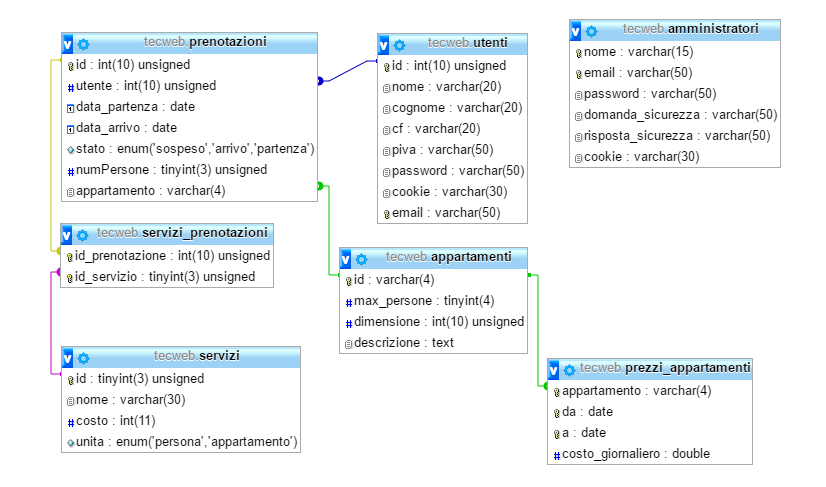
\includegraphics[scale=0.80]{images/Struttura_Database.png}
\end{figure} 

\subsubsection{Struttura del sito}
Le pagine visualizzabili dagli utenti ospiti o amministratori del sito sono descritte nel seguito.
\begin{itemize}
\item \textbf{index.php:} è la homepage del sito. Mostra una piccola descrizione del residence è la sua ubicazione; 
\item \textbf{login.php:} è la pagina contenente il form di login sia per l'utente amministratore che per gli utenti ospiti. Nel qual caso un utente ospite non abbia le credenziali di accesso tramite questa pagina ha la possibilità di registrarsi usufruendo dell'apposito form. Il sito prevede un unico account amministratore, motivo per il quale non ci si può registrare come amministratori ma soltanto come utenti normali;
\item \textbf{appartamenti.php:} è la pagina che contiene una descrizione della struttura del residence, con le tipologie degli appartamenti disponibili e vari servizi possibili;
\item \textbf{attrazioni.php:} è la pagina che contiene una descrizione delle attrazioni nelle zone limitrofi al residence;
\item \textbf{prenotazioni.php:} è la pagina che contiene la lista degli appartamenti che si possono prenotare. In caso l'utente non fosse ancora loggato verrà automaticamente alla pagina di login descritta in uno dei punti precedenti. In caso fosse già loggato invece verrà indirizzato alla pagina di conferma della prenotazione, ovvero la pagina del punto seguente;
\item \textbf{prenotazione.php:} come accennato nel punto precedente questa pagina richiede la conferma di una prenotazione. In questa pagina si possono aggiungere i servizi offerti dal residence alla propria prenotazione;
\item \textbf{contatti.php:} è la pagina che contiene i contatti del residence e le indicazioni da seguire per arrivarci;
\item \textbf{riepilogoPrenotazioni.php:} è la pagina che contiene il riepilogo delle prenotazioni degli utenti del sito;
\item \textbf{aggiuntaAppartamenti.php:} è una delle pagine accessibili solamente dall'utente amministratore contenente la lista degli appartamenti del residence con la possibilità di modificarli, usando un bottone che indirizza alla pagina del punto successivo, o di eliminarli. Oltre a questo l'amministratore ha anche la possibilità di aggiungere un nuovo appartamento usando l'apposito form;
\item \textbf{modificaAppartamento.php:} come accennato nel punto precedente questa pagina, anch'essa accessibile esclusivamente dall'utente amministratore, permette la modifica di un appartamento del residence;
\item \textbf{servizi.php:} è un'altra delle pagine a cui può accedere solamente l'amministratore e mette a disposizione la possibilità aggiungere un servizio per gli ospiti del residence e di consultare la lista degli stessi con anche la possibilità di eliminarli;
\item \textbf{gestionePrenotazioni.php:} come le pagine dei punti precedenti questa pagina riguarda il lato amministratore e si pone come una lista contenente tutte le prenotazioni che hanno fatto gli utenti ospiti del sito. Da questa pagina l'amministratore ha la possibilità di calcolare il costo totale della prenotazione cliccando sul bottone "Fattura" che lo indirizzerà alla pagina che verrà descritta nel punto seguente; 
\item \textbf{preventivi.php:} come accennato nel punto precedente l'utente amministratore accede a questa pagina per il calcolo del totale di una data prenotazione. Qua infatti saranno elencati sia i servizi aggiunti alla propria prenotazione che il totale del costo dell'appartamento dato dal costo giornaliero dello stesso moltiplicato per i giorni prenotati. 
\item \textbf{404.php:} questa pagina viene richiamata in caso un qualsiasi tipo di utente cercasse di accedere ad una pagina del sito non esistente. Per l'indirizzamento a questa pagina si è usato il file \textit{.htaccess} posizionato nella \textit{directory generale}.
\end{itemize}

\newpage
\subsection{Presentazione}
Il sito è stato progettato per avere un layout responsive, fluido, accessibile ed adattabile ad ogni dispositivo. Questo è stato possibile grazie all'uso di misure in \textit{em} e in percentuali quando le misure in questione riguardavano larghezze che dovevano essere adattate in base alla larghezza dello schermo. Grazie a questo tipo di progettazione il sito è accessibile anche da dispositivi mobile; dispositivi nei quali i blocchi vengono per lo più sovrapposti uno sopra l'altro, vista la ridotta larghezza dello schermo, invece di lasciarli flottanti e posizionati in modo spesso adiacente come nella modalità desktop. Una scelta progettuale ha portato alla decisione di non usare il breadcrumb; questa decisione è conseguenza del fatto che il sito ha una gerarchia di pagine che non supera profondità grado 2. Oltre a questo si è fatto in modo che se si tenta di accedere direttamente a tali pagine tramite link si viene catapultati nella pagina padre di profondità grado 1. Pagine nelle quali l'utente potrà capire dove si trova grazie alla colorazione differente del nome della pagina in cui si trova nel menu posizionato nel \textit{header}.

\subsection{CSS3}
Il \textit{CSS3} offre numerose possibilità per un web designer attento all'estetica della propria pagina. Le scelte adottate massimizzano non solo la retrocompatibilità del sito e dei contenuti ma anche dell'aspetto grafico. Le regole CSS3 vengono utilizzate per dare un aspetto attraente e maggiormente curato nei dettagli.

\subsection{JavaScript}
\textit{JavaScript} è stato utilizzato per fare controlli sui campi che l'utente inserisce o ha modo di modificare. Tutto questo per migliorare l'esperienza di navigazione dell'intero sito. Pur essendo questi controlli di utilità primaria la loro assenza, in caso di \textit{JavaScript} disabilitato, non comporta perdita di funzionalità o malfunzionamenti visto che i controlli  vengono rieseguiti tramite \textit{Php}.

\subsection{Php}
Gran parte delle pagine del nostro sito sono state realizzate con \textit{Php} per sfruttare la possibilità di effettuare controlli, siano essi sull'identità dell'utente siano essi sulla conformità dell'input che immette l'utente. Tutte le pagine a cui può accedere un utente o un amministratore sono in \textit{Php}, anche se il contenuto vero e proprio è strutturato usando \textit{Html}. Questo avviene grazie alla totale separazione tra quest'ultimo e il \textit{Php} che riesce bene usando il file \textit{gestoreHeader.php}, posizionato nella cartella \textit{php}, e le sue funzioni.

\subsection{XHTML}
Poichè non è possibile sapere i mezzi utilizzati dagli utenti si è optato per l'utilizzo di \textit{HTML Strict} per massimizzare la retrocompatibilità.

\newpage
\section{Accessibilità}
Il sito è stato pensato per essere facilmente utilizzabile dalla maggior utenza possibile. Per far questo si è cercato di:
\begin{itemize}
\item far sì che l'intero sito sia utilizzabile anche con \textit{JavaScript} disabilitato.
\item utilizzare solo colori "web safe", ovvero colori compatibili con tutti i browser.
\item utilizzare l'attributo "alt" per ogni immagine presente in modo da fornire un'alternativa testuale a questo tipo di contenuto che per un certo tipo di utenti non è visibile e che quindi potranno solo capire di cosa si tratta grazie agli \textit{Screen Reader}.
\item utilizzare l'attributo "xml:lang" e "lang" per identificare le parole in lingua straniera, in modo che gli \textit{Screen Reader} possano leggerle con la pronuncia esatta.
%\item utilizzare l'attributo "tabindex" per permettere una navigazione facilitata attraverso l'uso della sola tastiera.
%\item fornire all'inizio di ogni pagina un link che permetta agli utenti che fanno uso di \textit{Screen Reader} di saltare direttamente al contenuto della pagina.
\item dare titoli alle pagine che ne descrivessero l'argomento o la finalità il più possibile esaudiente.
\item tenere un struttura delle pagine il più possibile intuitiva e omogenea in tutte le pagine del sito.
\end{itemize}

\section{Validazione}
\subsection{XHTML Strict}
Per validare il codice \textit{XHTML 1.0 Strict} abbiamo utilizzato il validatore del W3C. Tale validatore è accessibile all'indirizzo:  \url{https://validator.w3.org/}.
\subsection{CSS3}
Per validare il codice \textit{CSS3} abbiamo utilizzato il validatore del W3C. Tale validatore è accessibile all'indirizzo:  \url{https://jigsaw.w3.org/css-validator/}.

\newpage
\section{Credenziali}
Per provare il sito si consiglia l'utilizzo degli account elencati in seguito.
\subsection{Credenziali utenti}
\begin{itemize}
\item \textbf{Email:} ab@gmail.com \textbf{Password:} abdelilah;
\item \textbf{Email:} teo@gmail.com \textbf{Password:} matteo;
\item \textbf{Email:} edo@gmail.com \textbf{Password:} edoardo.
\end{itemize}
\subsection{Credenziali amministratore}
\begin{itemize}
\item \textbf{Email:} admin@gmail.com \textbf{Password:} administrator;
\end{itemize}

\section{Ruoli}
\begin{itemize}
\item \textbf{Lahmer Abdelilah:} Php e HTML pagine di gestione appartamenti, Relazione;
\item \textbf{Maran Matteo:} Php, CSS, HTML;
\item \textbf{Zanon Edoardo:} JavaScript, Php, CSS, HTML;
\end{itemize}

\end{document}